\subsection{Thread Spawner}

\begin{figure}[H]
	\centering
	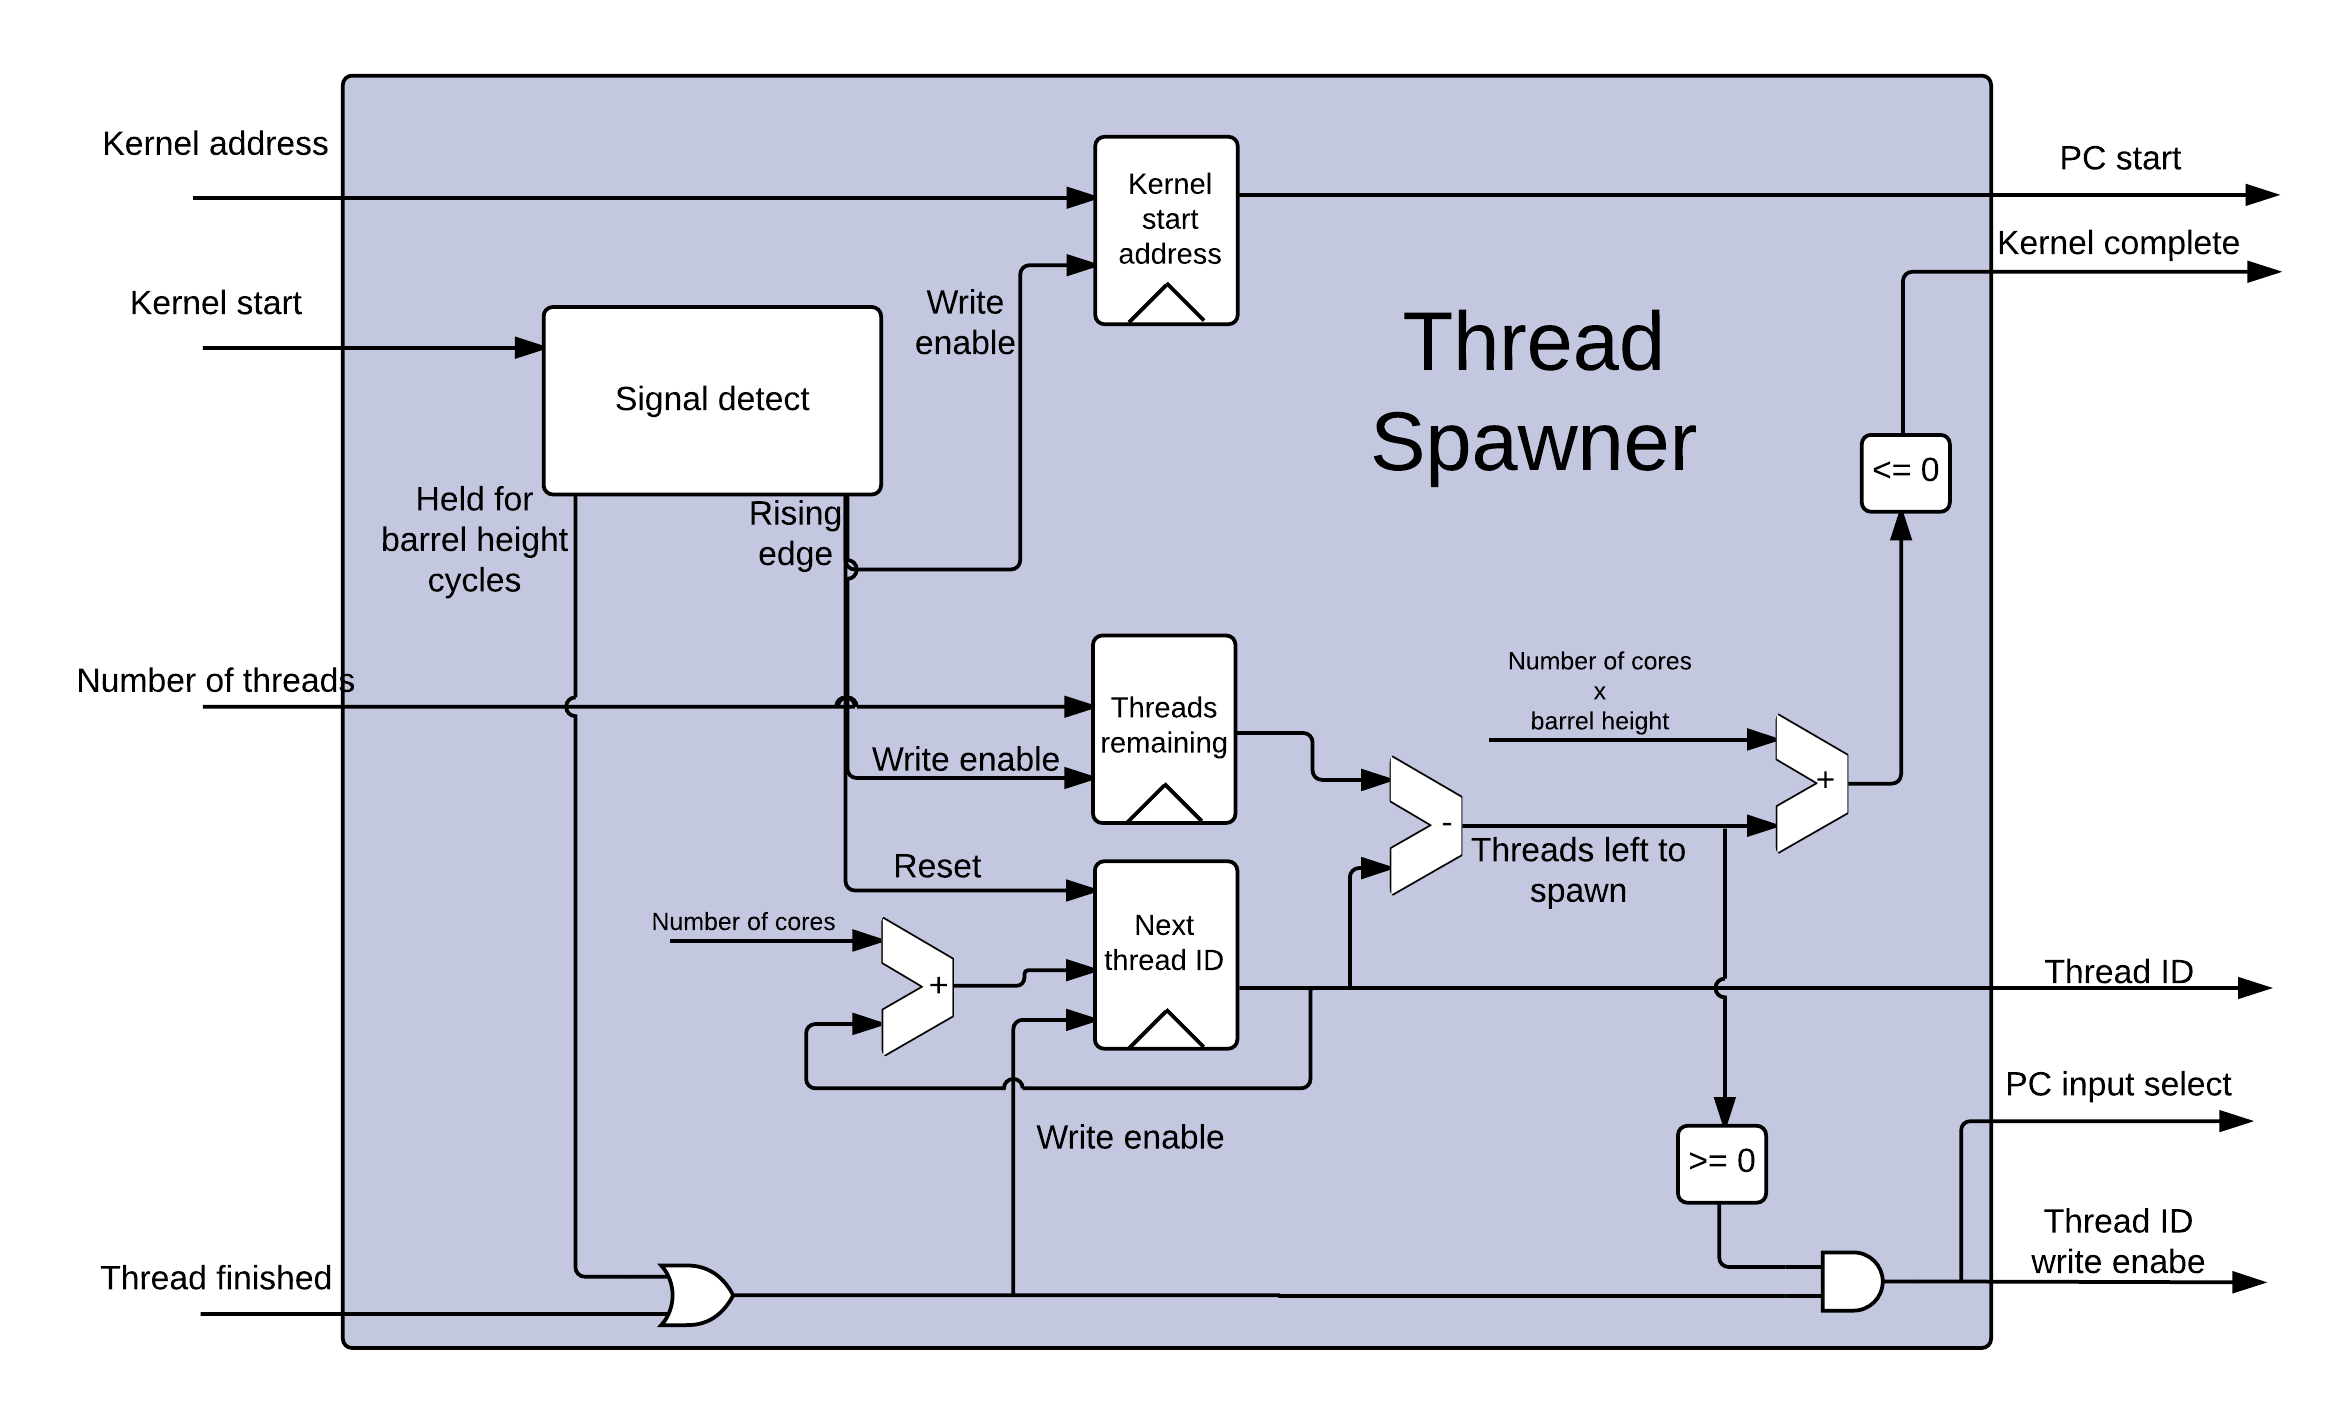
\includegraphics[width=\textwidth]{../gpu/diagrams/thread_spawner.png}
	\caption{Thread spawner and neighboring components}
	\label{fig:thread_spawner}
\end{figure}

The thread spawner is responsible for overseeing kernel execution.
It will spawn threads whenever necessary, handling thread setup and ensuring that the requested kernel is executed.
When all threads have finished executing, it will assert the kernel done signal, notifying the host program that computation has finished.

When a kernel invocation request is received, the thread spawner stores the provided base address of the kernel, the number of threads to spawn, and sets the next threadID register to zero.
Threads are spawned one warp at a time into the currently active barrel line.
Therefore, on kernel start the thread spawner will spawn threads untill the warp drive has made an entire rotation.

When a thread finishes execution, the control unit will assert the 'finished' signal to the thread spawner.
If there are threads left to spawn, the currently active barrel row will be filled with a new warp of threads.

But what does the spawning of a warp of threads actually entail?
All threads need an unique threadID.
If the ID of the next thread to spawn is 4, and we have 4 processor cores,
core 0 will write threadID 4 to its threadID register, core 1 threadID 5, and so forth.
The next threadID is then incremented by the warp size, increasing from 4 to 8.

If the warp is spawned into barrel line zero, the program counter will be reset to the kernel base address, and the first instruction of the kernel will start trickling down the barrel lines.
A new warp of threads has been spawned!
